\chapter{Objekterkennung}
\label{ch:Objekterkennung}
\sectionmark{Objekt}

Die Objekterkennung spielt eine fundamentale Rolle für die autonome Navigation des Duckiebots, da sie die Wahrnehmung relevanter Objekte in der Umgebung ermöglicht. Im Rahmen dieses Projekts wurde ein vortrainiertes YOLOv8n-Modell (You Only Look Once, Version 8 nano) eingesetzt, um verschiedene Objektklassen in Echtzeit zu identifizieren und deren Position im Kamerabild zu lokalisieren. Dieses Modell wurde in der \texttt{detect\_object\_node} implementiert und lieferte die Grundlage für die Entscheidungsfindung in mehreren nachfolgenden Herausforderungen.

\section{YOLOv8n und die \texttt{detect\_object\_node}}
\sectionmark{YOLOv8n}

YOLOv8n ist eine \ac{CNN}-Architektur, die für ihre hohe Geschwindigkeit und Genauigkeit bei der Objektdetektion bekannt ist. Das \enquote{nano}-Modell zeichnet sich durch seine geringe Größe und Effizienz aus, was es ideal für den Einsatz auf ressourcenbeschränkten Systemen wie dem Duckiebot macht. Das Modell wurde auf einem Datensatz trainiert, der spezifische Duckietown-Objekte wie \enquote{Duckies} (Enten), \enquote{Duckiebots} (andere Fahrzeuge) sowie \enquote{freeSlot} und \enquote{occupiedSlot} (freie und belegte Parklücken) umfasste. Die Leistungsfähigkeit des Modells, wie die Konfusionsmatrix, Präzisions-Recall-Kurven und weitere Metriken zeigen, ist in Abbildung~\ref{fig:yolo_results} detailliert dargestellt.

Die DetectParkingSlotNode ist die zentrale Komponente, die für die Verarbeitung der Kamerabilder und die Anwendung des YOLOv8-Modells zuständig ist. Ihr grundlegender Ablauf ist in Abbildung~\ref{fig:object_detection_flow} illustriert. Die Node abonniert komprimierte Kamerabilder vom Topic \texttt{camera\_node/image/compressed} und führt die folgenden Schritte aus:
\begin{enumerate}
    \item \textbf{Dekompression und Vorverarbeitung:} Das empfangene CompressedImage-Nachricht wird mittels CvBridge in ein OpenCV-Bildformat (bgr8) konvertiert.
    \item \textbf{Inferenz mit YOLOv8n:} Das Bild wird dem geladenen YOLOv8n-Modell (self.\_model) zugeführt. Die Ergebnisse (results.boxes) enthalten eine Liste von Detektionen, wobei jede Detektion Informationen über die Bounding Box (xyxy), eine Konfidenzbewertung (conf) und die Klassenzugehörigkeit (cls) des Objekts enthält.
    \newpage
    \item \textbf{Klassifizierung und Filterung:} Die rohen Detektionen werden nach ihren Labels (\enquote{Duckie}, \enquote{Bot}, \enquote{Slot}) sowie vordefinierten Konfidenzschwellen (\texttt{conf\_threshold\_duckie}, \texttt{conf\_threshold\_bot}, \texttt{conf\_threshold\_slot} aus der YAML-Konfiguration) gefiltert. Für die Unterscheidung zwischen freeSlot und \texttt{occupiedSlot} wird eine \ac{IoU}-Berechnung (compute\_iou) durchgeführt, um zu prüfen, ob ein erkanntes Slot-Objekt eine Überlappung mit einem Duckie oder Bot aufweist, und somit als \texttt{occupiedSlot} klassifiziert werden kann.
    \item \textbf{Region of Interest Filterung:} Mithilfe von dynamisch aus der Konfiguration geladenen Polygonen (\texttt{mask\_lane}, \texttt{mask\_right}, \texttt{mask\_bot}) wird überprüft, ob die detektierten Objekte in relevanten Bereichen des Kamerabildes liegen (is\_in\_mask). Dies hilft, Fehlalarme zu reduzieren und nur Objekte zu berücksichtigen, die für die Fahrstrategie relevant sind.
    \item \textbf{Temporale Stabilität und Auswahl:} Die Node nutzt deque-Objekte (\texttt{self.history\_duckie\_lane}, etc.) zur historischen Speicherung von Detektionsstatus über mehrere Frames. Ein Objekt wird nur als präsent bestätigt, wenn die über eine konfigurierbare Anzahl von Frames gemittelte Konfidenz (\texttt{confidence\_temporal}) einen bestimmten Schwellenwert überschreitet. Innerhalb jeder Klasse wird in der Regel das nächste Objekt (basierend auf der Y-Koordinate am unteren Rand der Bounding Box) ausgewählt.
    \item \textbf{Publikation der Ergebnisse:} Die Informationen der erkannten Objekte werden über spezifische \ac{ROS}-Topics veröffentlicht, sodass andere Nodes im System darauf zugreifen und ihre Entscheidungen basierend auf diesen Daten treffen können. Eine beispielhafte Detektion im Betrieb ist in Abbildung~\ref{fig:detect_object} dargestellt.
    \begin{itemize}
        \item /detect/object/duckieNearestBB: Bounding Box der nächsten Ente in der Fahrspur.
        \item /detect/object/duckieNearestRightBB: Bounding Box der nächsten Ente in der rechten Spur (relevant für Ausweichmanöver).
        \item /detect/object/botNearestBB: Bounding Box(en) des/der nächsten Duckiebot(s).
        \item /detect/object/parkingBB: Bounding Box der nächsten freien Parklücke.
        \item /detect/object/parkingOccupiedBB: Bounding Box der nächsten belegten Parklücke.
        \item /detect/object/image: Annotiertes Bild mit den erkannten Bounding Boxes und Klassennamen zu Debugging-Zwecken.
    \end{itemize}
\end{enumerate}

Die temporale Glättung durch die Verwendung der deque-Historien und die konfigurierbaren Schwellenwerte für Konfidenz und \ac{IoU} sind entscheidende Maßnahmen, um die Robustheit der Objektdetektion zu erhöhen und Flackern von Detektionen zu reduzieren.

\begin{figure}[htbp]
    \centering
    \begin{subfigure}{\VarPicWidthF}
        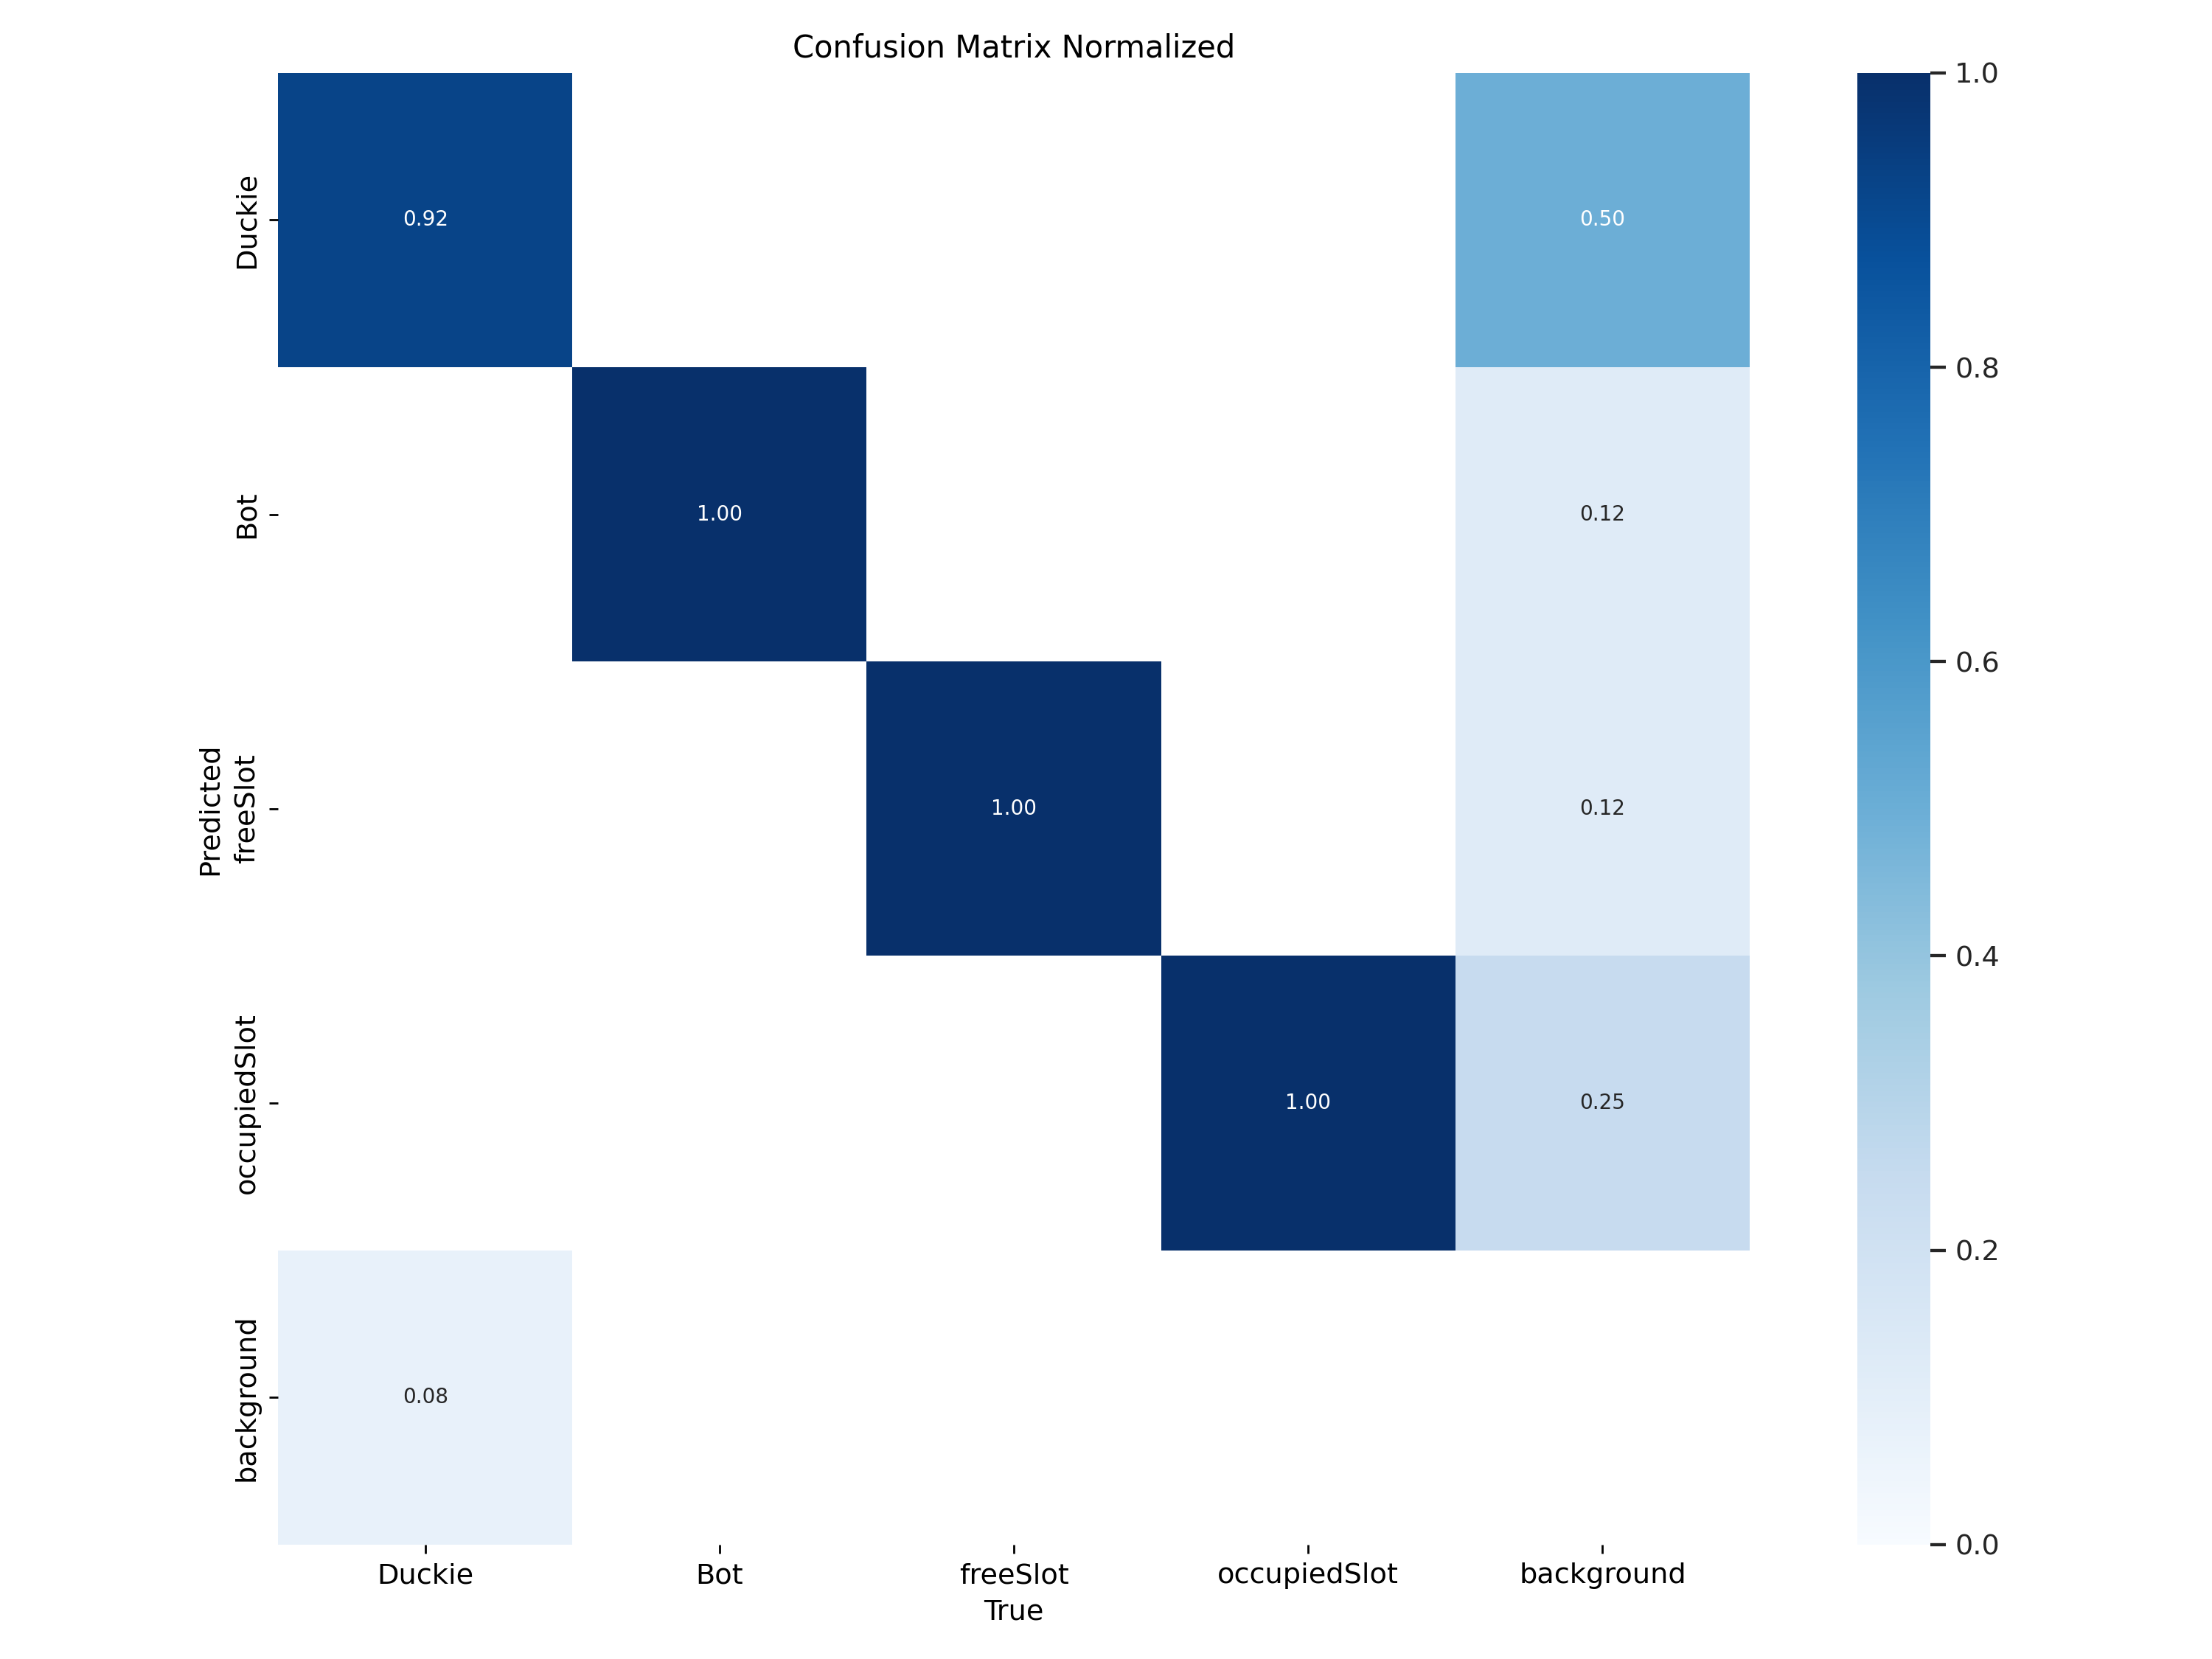
\includegraphics[width=\textwidth]{Figures/png/confusion_matrix.png}
        \caption{Konfusionsmatrix}
        \label{fig:confusion_matrix}
    \end{subfigure}
    \begin{subfigure}{\VarPicWidthF}
        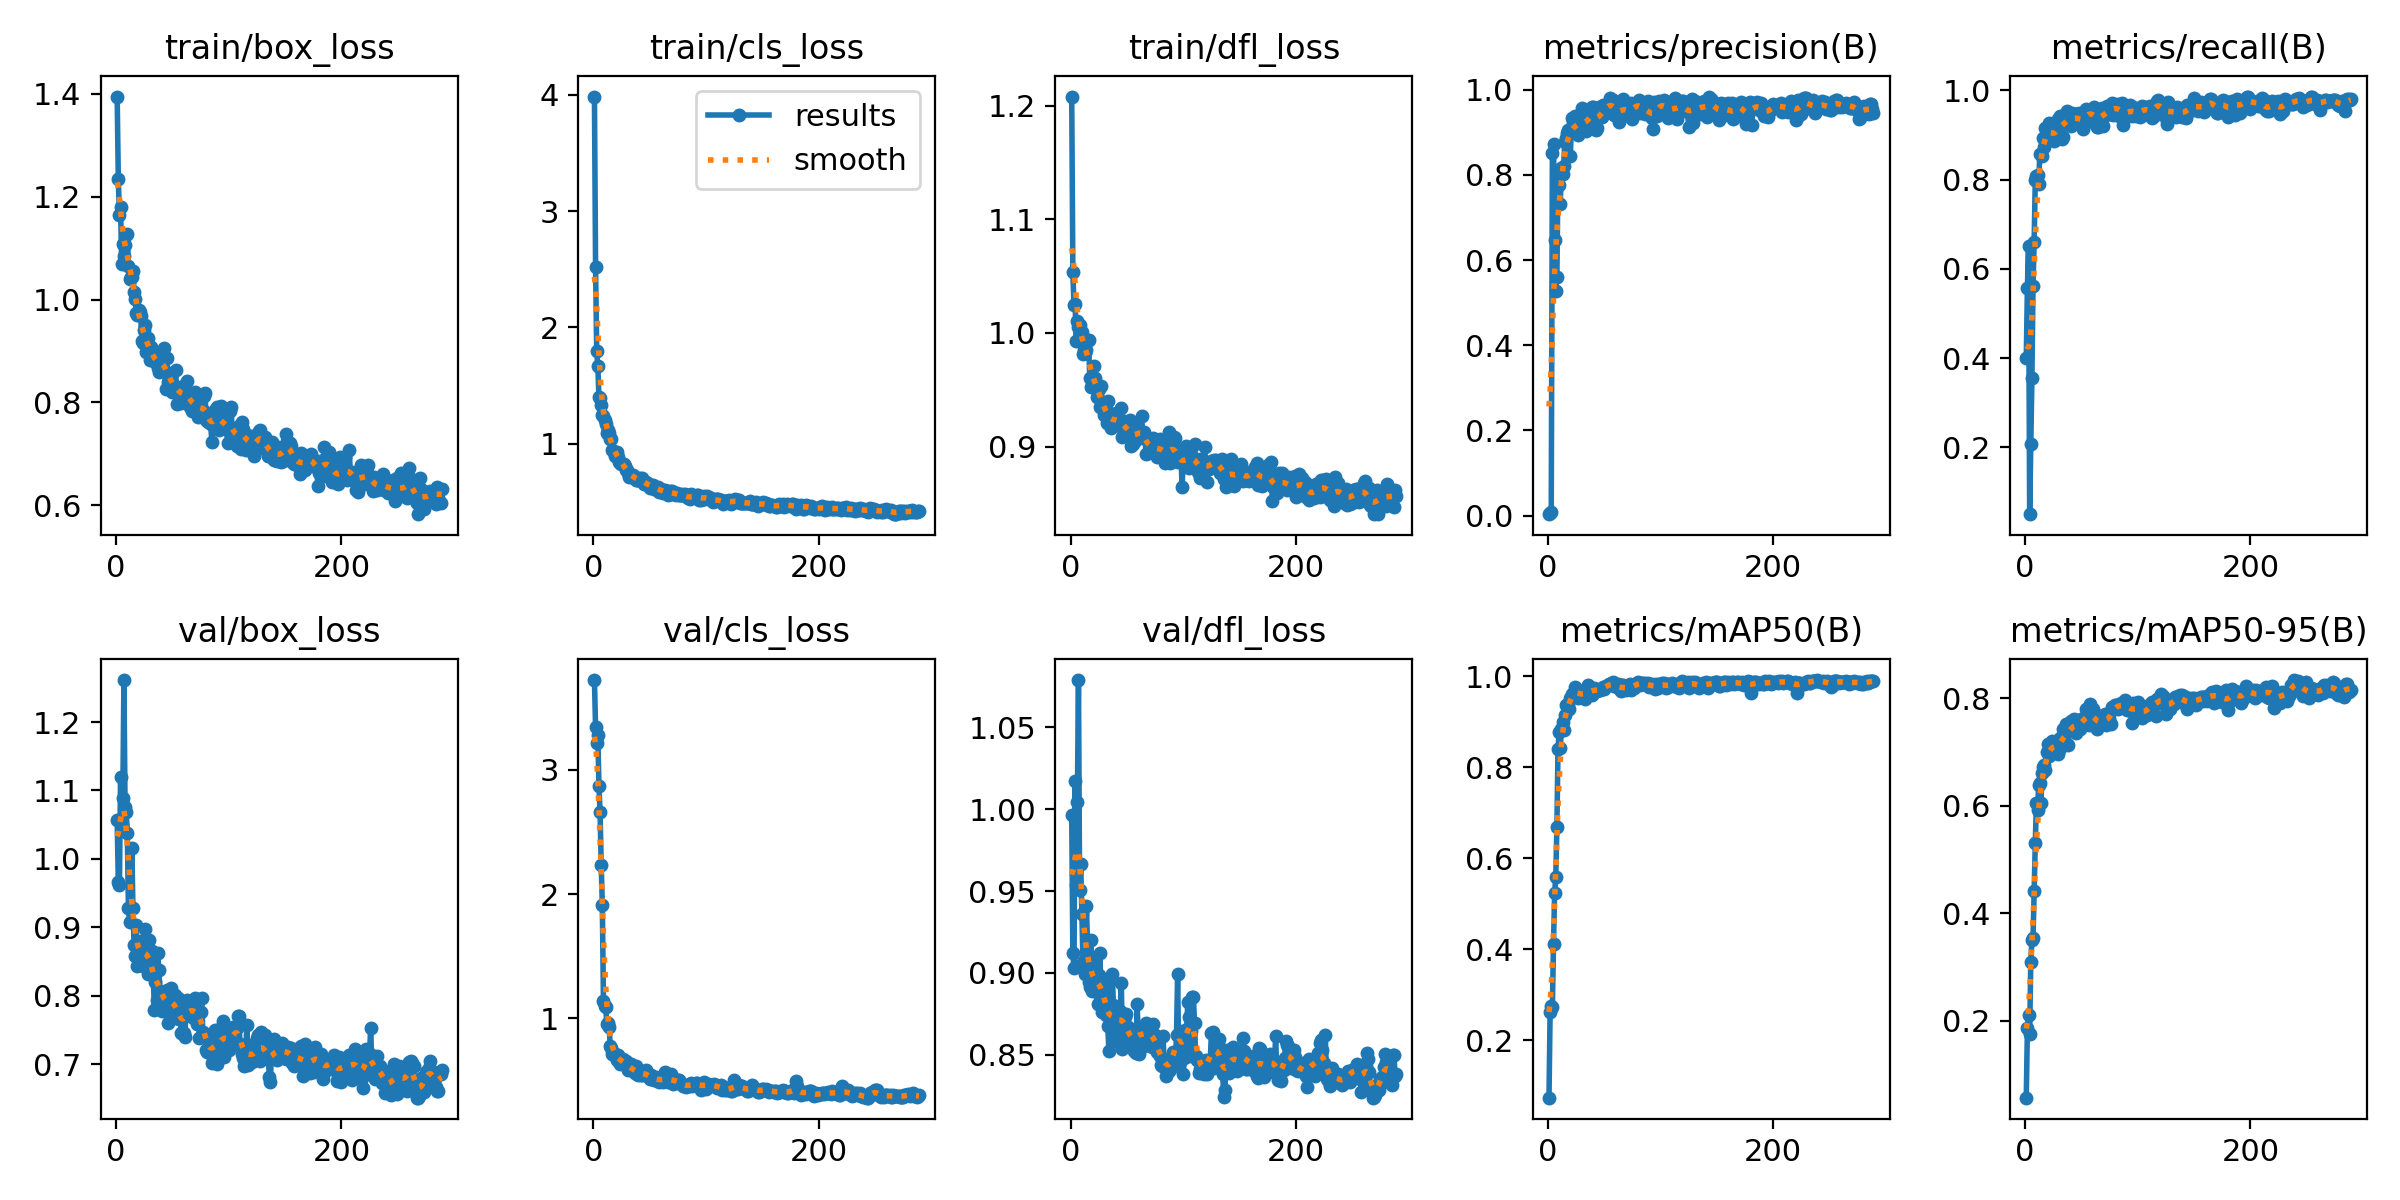
\includegraphics[width=\textwidth]{Figures/png/results.png}
        \caption{Ergebnisse}
        \label{fig:confusion_matrix}
    \end{subfigure}
    \begin{subfigure}{\VarPicWidthF}
        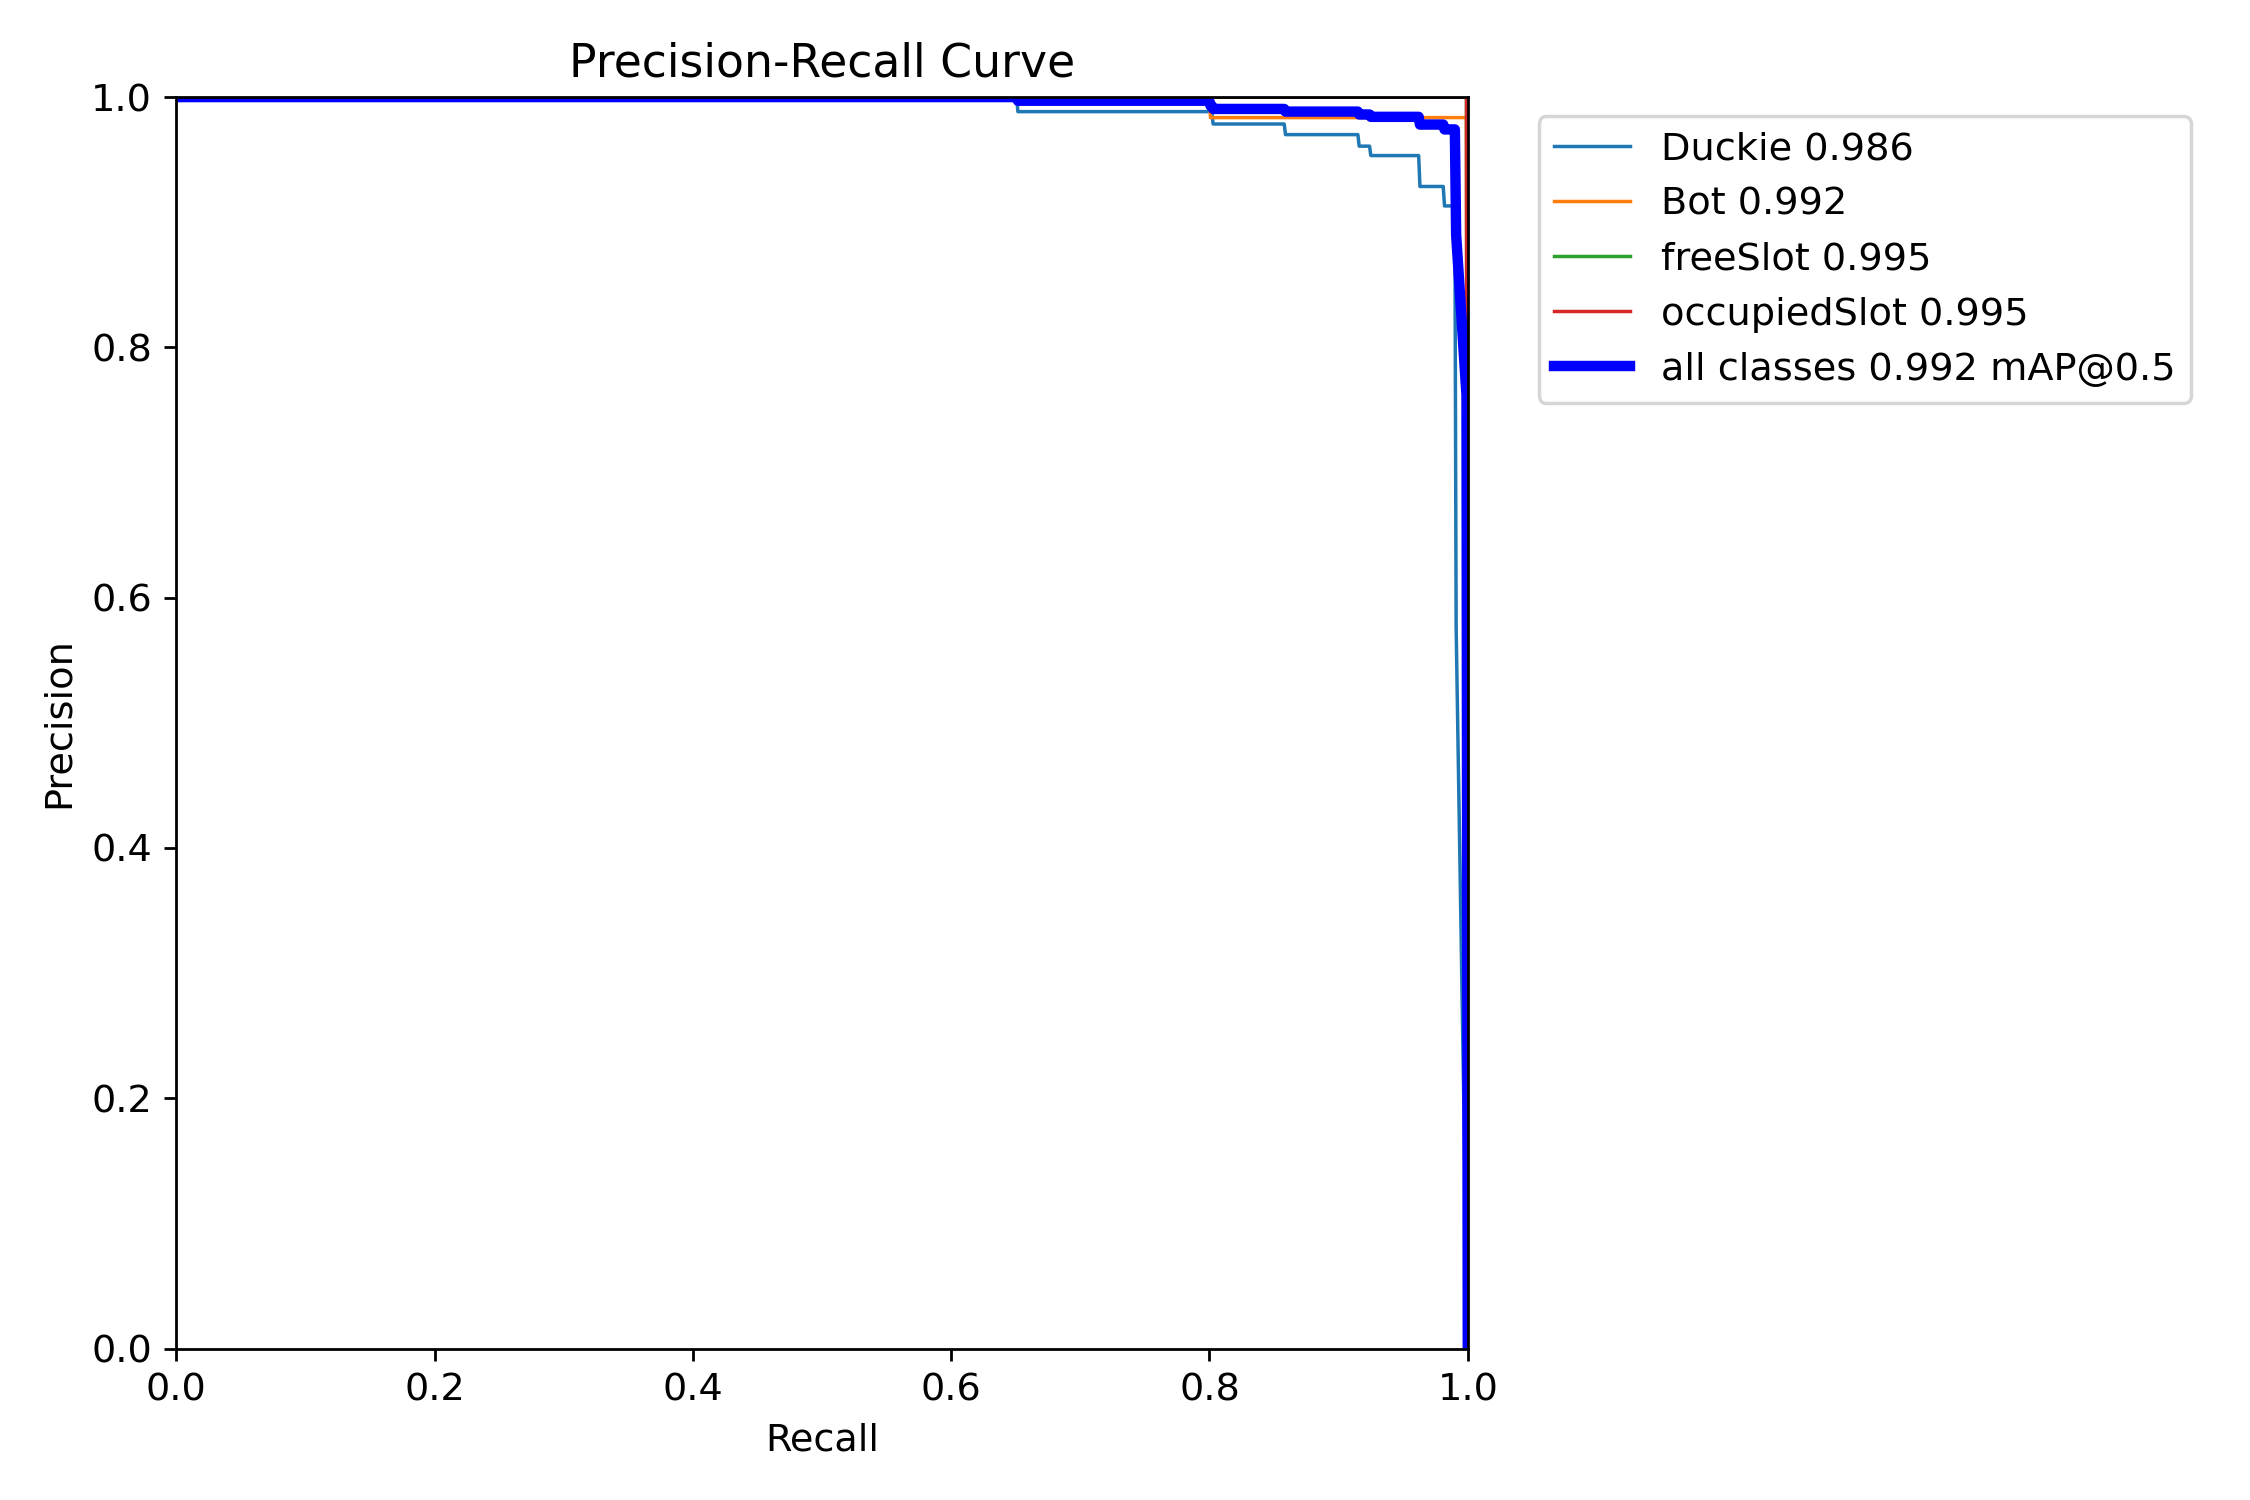
\includegraphics[width=\textwidth]{Figures/png/PR_curve.png}
        \caption{PR-Kurve}
        \label{fig:confusion_matrix}
    \end{subfigure}
    \begin{subfigure}{\VarPicWidthF}
        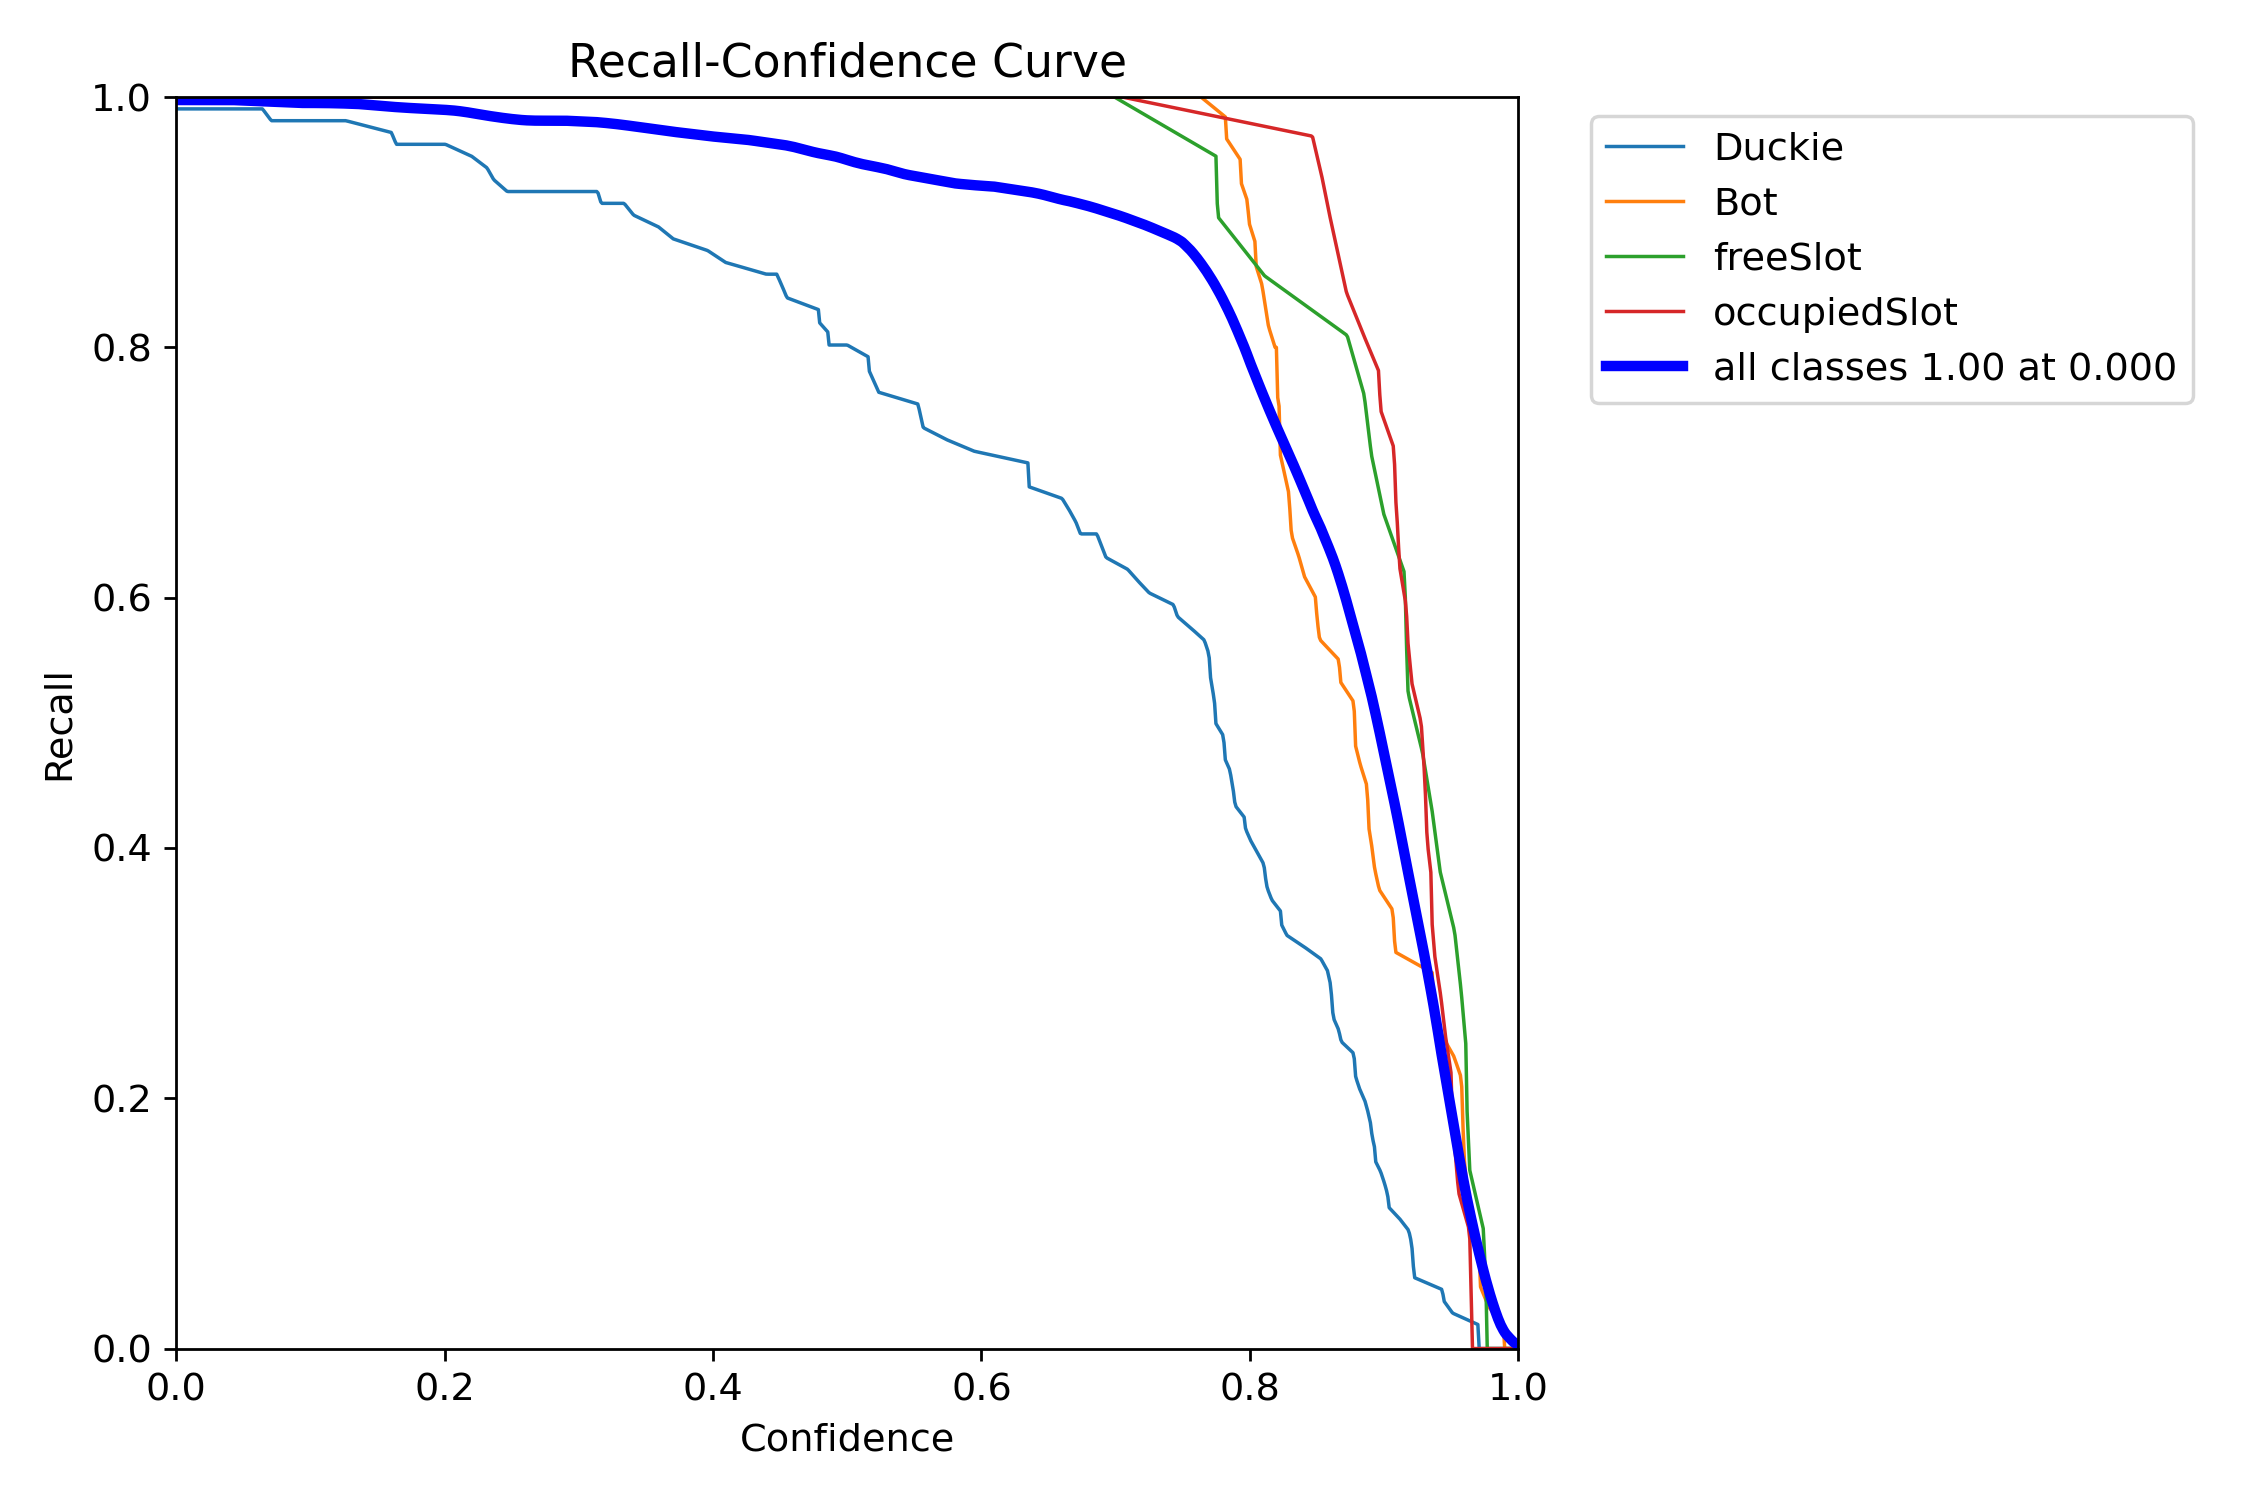
\includegraphics[width=\textwidth]{Figures/png/R_curve.png}
        \caption{R-Kurve}
        \label{fig:confusion_matrix}
    \end{subfigure}
    \caption{Ergebnisse des YOLOv8n-Trainings}
    \label{fig:yolo_results}
\end{figure}

\begin{figure}[hptb]
    \centering
    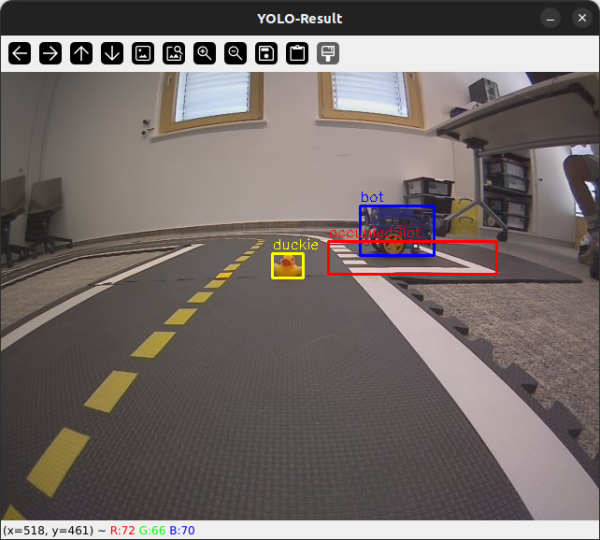
\includegraphics[width=0.7\textwidth]{Figures/png/detect_objects.png}
    \caption{Beispielbild mit erkannten Objekten im Betrieb (Bounding Boxes und Labels).}
    \label{fig:detect_object}
\end{figure}

\newpage



\section{Ablaufdiagramm der Objekterkennung}
\label{sec:object_detection_flow}
\sectionmark{Ablauf}

Das folgende Ablaufdiagramm in Abbildung~\ref{fig:object_detection_flow} illustriert den internen Prozess der \texttt{detect\_object\_node}.

\begin{figure}[hptb]
    \centering
    \begin{subfigure}{\VarPicWidthE}
        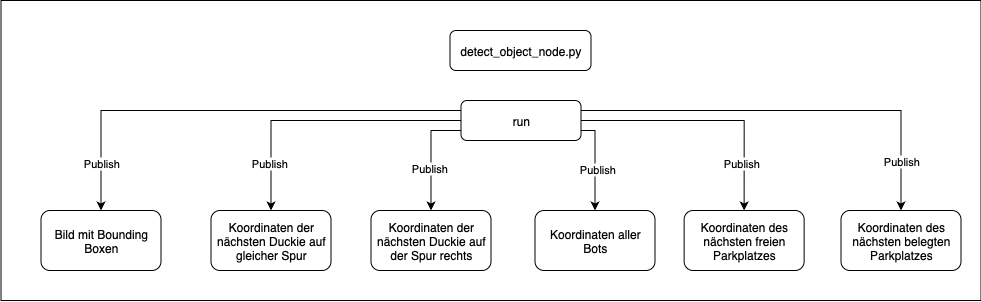
\includegraphics[width=\textwidth]{Figures/png/Struktur_YoloNode.png}
        \caption{Struktur der Detect Object Node}
        \label{fig:object_detection_structur}
    \end{subfigure}
    \begin{subfigure}{\VarPicWidthB}
        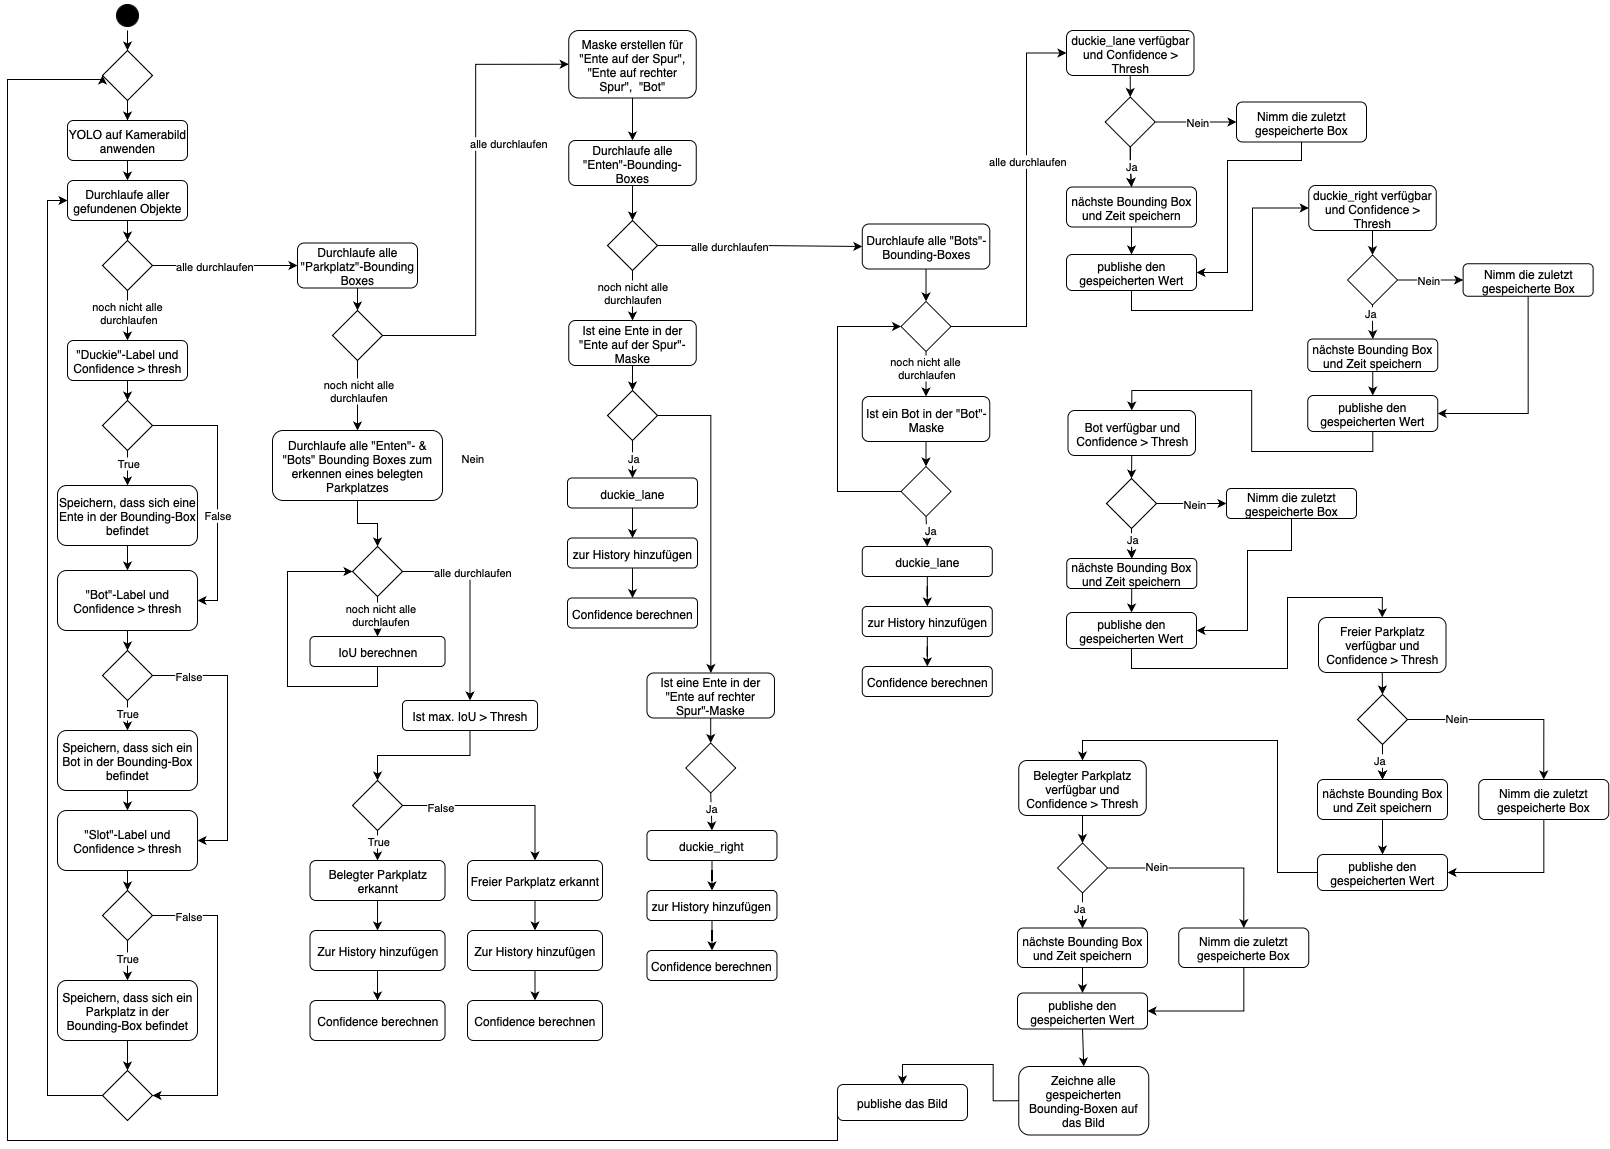
\includegraphics[width=\textwidth]{Figures/png/Ablaufdiagramm_YOLO.png}
        \caption{Ablaufdiagramm der Detect Object Node}
        \label{fig:object_detection_flow}
    \end{subfigure}
    \caption{\texttt{object\_detection\_node}}
    \label{fig:object_detection_node}
\end{figure}

Die Node beginnt mit der Initialisierung der \ac{ROS}-Kommunikation und dem Laden des vortrainierten YOLOv8n-Modells sowie der Konfigurationsparameter. In einer Endlosschleife wird kontinuierlich auf neue Kamerabilder gewartet. Sobald ein Bild empfangen wird, wird es dekomprimiert und an das YOLO-Modell übergeben. Die vom Modell zurückgegebenen Detektionen (Bounding Boxes, Konfidenzen, Klassen) werden anschließend verarbeitet. Hierbei werden nicht relevante Detektionen (z.B. zu geringe Konfidenz, außerhalb der Maske) gefiltert und, falls relevant, die Überlappung mit anderen Objekten (für \texttt{occupiedSlot}) bewertet. Die Relevanz der Detektion über die Zeit wird durch historische Puffer (deque) beurteilt. Die final als relevant befundenen Objekte werden identifiziert (z.B. der nächste Duckie, der nächste freie Parkplatz), und ihre Bounding Box-Informationen werden dann über dedizierte \ac{ROS}-Topics an andere Nodes im System veröffentlicht, um dort für Steuerungsentscheidungen genutzt zu werden. Optional kann auch ein visualisiertes Bild mit den Bounding Boxes zur Fehlerbehebung ausgegeben werden.



\section{Technische Umsetzung im Code}
\label{sec:object_detection_code}
\sectionmark{Code}

Die \texttt{detect\_object\_node} ist die primäre Implementierung der Objekterkennung. Der vollständige Python-Code kann in~\cite{QuackSquad}, Funktion \texttt{detect\_object\_node.py} eingesehen werden.

\subsection{Initialisierung und Konfiguration}
Beim Start der Node (\texttt{\_\_init\_\_}-Methode) werden grundlegende \ac{ROS}-Kommunikationsmittel und Parameter initialisiert. Dazu gehören:
\begin{itemize}
    \item Die Initialisierung der DTROS-Node und das Abrufen des Fahrzeugnamens (\texttt{\_vehicle\_name}).
    \item Die Einrichtung von CvBridge für die Konvertierung von \ac{ROS}-Bildnachrichten in OpenCV-Formate.
    \item Die Initialisierung von deque-Objekten (\texttt{history\_duckie\_lane}, etc.) für die temporale Glättung der Detektionsergebnisse.
    \item Das Laden des YOLOv8n-Modells aus dem angegebenen Asset-Pfad.
    \item Das Einlesen der Konfigurationsparameter (z.B. \texttt{conf\_threshold\_duckie}, \texttt{iou\_threshold}, \texttt{mask\_lane} Polygone) aus der detect\_duckieBotSlot.yaml-Datei.
    \item Die Einrichtung von Publishern für die verschiedenen Bounding Box-Informationen (z.B. \texttt{pup\_duckieNearestBB}, \texttt{pup\_parkingBB}, \texttt{pup\_botNearestBB}) und einen Publisher für das annotierte Debug-Bild (\texttt{pup\_image}).
    \item Die Registrierung des Subscribers \texttt{sub\_image} für komprimierte Kamerabilder.
\end{itemize}
Die Methoden \texttt{get\_polygon}, \texttt{compute\_iou} und \texttt{is\_in\_mask} dienen als Hilfsfunktionen zur Verarbeitung der Masken und zur Überlappungsberechnung, die in der Hauptlogik verwendet werden.

\subsection{Bild- und Objekterkennungsprozess (\texttt{run}-Methode)}
Die Kernlogik der Node befindet sich in der \texttt{run}-Methode, die in einer Schleife kontinuierlich ausgeführt wird.
\begin{enumerate}
    \item Bildverarbeitung: Bei Verfügbarkeit eines neuen Bildes (bereitgestellt über die \texttt{cbDetectObjects}-Callback-Funktion) wird dieses für die YOLO-Inferenz verwendet.
    \item YOLO-Inferenz und Roh-Detektionen: Das \texttt{self.\_model(self.cv\_image, verbose=False)[0]} führt die Objektdetektion durch. Die zurückgegebenen boxes enthalten die Bounding Box-Koordinaten, Konfidenzwerte und Klassifikationen.
    \item Klassenspezifische Sortierung: Die erkannten Objekte werden basierend auf ihren Labels in Listen für Duckies, Bots und Slots vorsortiert.
    \item Slot-Klassifizierung (Free/Occupied): Für die erkannten Slots wird mittels der \texttt{compute\_iou}-Methode geprüft, ob diese mit einem Duckie oder Bot überlappen. Überschreitet die \ac{IoU} einen Schwellenwert (\texttt{iou\_threshold}), wird der Slot als \texttt{occupiedSlot} klassifiziert, ansonsten als freeSlot. Dies ist entscheidend für das Parkmanöver in Challenge 4 (siehe Kapitel~\ref{ch:Challenge_4}).
    \item Masken- und Temporale Filterung: Die \texttt{is\_in\_mask-Methode} wird verwendet, um zu prüfen, ob die Objekte innerhalb der vordefinierten \texttt{mask\_lane}, \texttt{mask\_right} oder \texttt{mask\_bot}-Polygone liegen. Die deque-Historien (\texttt{history\_duckie\_lane}, etc.) werden aktualisiert, um die zeitliche Präsenz eines Objekttyps zu verfolgen. Nur Detektionen, deren temporale Konfidenz (\texttt{conf\_duckie}, etc.) über dem \texttt{confidence\_temporal}-Schwellenwert liegt, werden für die Ausgabe in Betracht gezogen.
    \item Verwaltung und Publikation der \enquote{Nearest} Bounding Boxes: Für jede relevante Objektklasse (Duckie in Fahrspur, Duckie rechts, Bot, freier Slot, belegter Slot) wird die nächstgelegene (basierend auf der Y-Koordinate am unteren Rand der Bounding Box) oder relevanteste Detektion ausgewählt. Diese Bounding Box-Informationen werden als \texttt{Float64MultiArray}-Nachrichten auf den jeweiligen \ac{ROS}-Topics publiziert (\texttt{pup\_duckieNearestBB}, \texttt{pup\_parkingBB}, etc.). Ein \texttt{timeout\_sec} sorgt dafür, dass die letzte bekannte Detektion für kurze Zeit weiter publiziert wird, auch wenn sie in einem Frame nicht mehr erkannt wurde, um Flackern zu minimieren.
    \item Visualisierung (Debugging): Ein annotiertes Bild, das die Bounding Boxes der aktuell erkannten und publizierten Objekte zeigt, wird über \texttt{pup\_image} veröffentlicht, was für das Debugging während der Entwicklung sehr hilfreich ist.
\end{enumerate}

\subsection{Robustheitsmaßnahmen}
Die Zuverlässigkeit der Objekterkennung unter realen Bedingungen wird durch mehrere in dieser Node implementierte Maßnahmen erheblich verbessert:
\begin{itemize}
    \item Konfidenzschwellen: Nur Detektionen mit einer Konfidenz über den in der Konfigurationsdatei festgelegten Schwellenwerten (\texttt{conf\_threshold\_duckie}, \texttt{conf\_threshold\_bot}, \texttt{conf\_threshold\_slot}) werden berücksichtigt, um Fehlalarme zu minimieren.
    \item Regionale Masken (\ac{ROI}): Die aus der Konfiguration geladenen Polygone (\texttt{mask\_lane}, \texttt{mask\_right}, \texttt{mask\_bot}) definieren spezifische Bereiche im Kamerabild. Nur Objekte, deren Zentrum innerhalb dieser Masken liegt, werden verarbeitet, was die Relevanz der Detektionen erhöht und Störungen durch irrelevante Objekte im Hintergrund vermeidet.
    \item Temporale Glättung: Die Verwendung von deque-Historien zur Aggregation des Detektionsstatus über mehrere Frames hinweg ermöglicht eine zeitliche Glättung. Ein Objekt wird nur dann als kontinuierlich anwesend betrachtet, wenn es über eine definierte Anzahl von Frames hinweg stabil erkannt wird, was die Robustheit gegenüber kurzzeitigen Detektionsaussetzern oder -fehlern erhöht (\texttt{confidence\_temporal}).
    \newpage
    \item \ac{IoU}-basierte Slot-Klassifizierung: Die präzise Unterscheidung zwischen freeSlot und \texttt{occupiedSlot} mittels Intersection over Union zwischen Slot- und Objekt-Bounding Boxes ist eine robuste Methode, um den Status eines Parkplatzes zu bestimmen.
    \item Detektions-Timeout: Der \texttt{timeout\_sec} (z.B. 0.1 Sekunden) sorgt dafür, dass eine zuletzt erkannte Bounding Box für eine kurze Dauer weiter publiziert wird, auch wenn das Objekt im aktuellen Frame nicht erkannt wurde. Dies überbrückt kurze Detektionsaussetzer und führt zu einem stabileren Verhalten der konsumierenden Nodes.
\end{itemize}

Die DetectParkingSlotNode stellt somit eine leistungsfähige und flexible Komponente dar, die andere Module des Duckiebot-Systems mit essenziellen Informationen über die Umgebung versorgt und die Grundlage für komplexere Navigationsentscheidungen bildet.